\section{Teoría de la Complejidad Computacional}

``A veces la respuesta es tan simple que da miedo, pero encontrarla es un infierno''. - Agente K (Hombres de Negro, 1997).

Planteamos formalmente el Problema del Juego de las Piedras en su versión de decisión: \textit{Dado un tablero de $n \times m$ celdas donde cada celda está vacía u ocupada por una piedra verde o celeste, ¿es posible sacar piedras de tal forma que cada fila tenga al menos una piedra y cada columna no tenga piedras de ambos colores?}

Si alguien nos da una posible solución $S$ (el tablero resultante despues de remover las piedras), a esa propuesta la llamamos \textit{certificado}. A priori no sabemos la correctitud de éste mismo, pero podemos verificarla con un algoritmo validador: el \textit{certificador}. Para asi verificar si cumple con todas las reglas.

Comunmente en los algoritmos implementados analizamos la complejidad temporal y espacial para medir cuánto tarda un algoritmo y cuánta memoria consume. Ahora, cuando pasamos de algoritmos polinómicos a algoritmos exponenciales, la barrera del tiempo se vuelve intratable (Tabla \ref{table: tabla1}).

\begin{table}[H]
    \centering
    \caption{Tiempos de ejecución aproximados de distintos órdenes de complejidad según el tamaño de entrada $n$, asumiendo un procesador que ejecuta un millón de instrucciones de alto nivel por segundo.}
    \renewcommand{\arraystretch}{1.3}
    \begin{tabular}{|l|l|l|l|l|l|l|l|}
    \hline
        Tamaño $n$ & $n$ & $n\log_{2}{n}$ & $n^{2}$ & $n^{3}$ & $1.5^{n}$ & $2^{n}$ & $n!$ \\ \hline
        $n = 10$ & $< 1$ seg & $< 1$ seg & $< 1$ seg & $< 1$ seg & $< 1$ seg & $< 1$ seg & 4 seg \\ \hline
        $n = 30$ & $< 1$ seg & $< 1$ seg & $< 1$ seg & $< 1$ seg & $< 1$ seg & 18 min & $10^{25}$ años \\ \hline
        $n = 50$ & $< 1$ seg & $< 1$ seg & $< 1$ seg & $< 1$ seg & 11 min & 36 años & muy largo \\ \hline
        $n = 100$ & $< 1$ seg & $< 1$ seg & $< 1$ seg & 1 seg & 12.892 años & $10^{17}$ años & muy largo \\ \hline
        $n = 1.000$ & $< 1$ seg & $< 1$ seg & 1 seg & 18 min & muy largo & muy largo & muy largo \\ \hline
        $n = 10.000$ & $< 1$ seg & $< 1$ seg & 2 min & 12 días & muy largo & muy largo & muy largo \\ \hline
        $n = 100.000$ & $< 1$ seg & 2 seg & 3 horas & 32 años & muy largo & muy largo & muy largo \\ \hline
        $n = 1.000.000$ & 1 seg & 20 seg & 12 días & 31.710 años & muy largo & muy largo & muy largo \\ \hline
    \end{tabular}
    \label{table:tabla1}
\end{table}

\subsection{Polinomialidad, NP, NP-Completitud y Reducciones}

Los problemas de decisión que pueden resolverse mediante un algoritmo en tiempo polinomial pertenecen al conjunto $\mathcal{P}$. Por otro lado, todo problema de decisión para el cual, dada una solución candidata (certificado), se puede verificar su validez en tiempo polinomial mediante un certificador eficiente, pertenece al conjunto $\mathcal{NP}$. Y nos podemos dar cuenta que, $\mathcal{P} \subseteq \mathcal{NP}$: si podemos resolver un problema desde cero en tiempo polinomial, también podemos verificar una solución ignorando el certificado y resolviéndolo nosotros mismos en tiempo polinomial.

En las Ciencias de la Computacion, hay una pregunta que hasta el día de hoy no se pudo responder: ¿se cumple que $\mathcal{P} = \mathcal{NP}$? Lo que muchos piensan (y lo de sentido común) es que $\mathcal{P} \neq \mathcal{NP}$. Que verificar la validez de una solución es mas fácil que encontrarla desde cero. Si llegara a demostrarse que $\mathcal{P} = \mathcal{NP}$, el impacto en el mundo seria tremendo, desde una optimización perfecta hasta la ruptura inmediata de toda la criptografia moderna.

Dentro de este universo definimos dos clases fundamentales:
\begin{itemize}
    \item Un problema $X$ es \textbf{NP-Hard} si todo problema $Y \in \mathcal{NP}$ puede reducirse polinomialmente a $X$ ($\forall Y \in \mathcal{NP}, Y \leq_P X$). Es decir, $X$ es \textit{al menos tan difícil} como cualquier problema de $\mathcal{NP}$.
    \item Un problema $X$ es \textbf{NP-Completo} si cumple al mismo tiempo dos condiciones: $X \in \mathcal{NP}$ y $X \in \text{NP-Hard}$.
\end{itemize}

Para demostrar que un problema nuevo $X$ es NP-Completo sin tener que reducir todos los problemas de $\mathcal{NP}$ uno por uno, usamos la transitividad de las \textbf{reducciones polinomiales} ($\leq_P$). Si agarramos un problema $Y$ que ya sabemos que es NP-Completo y demostramos que $Y \leq_P X$, probamos que si existiera una ``caja negra'' capaz de resolver $X$ en tiempo polinomial, podríamos transformar cualquier instancia de $Y$ en una instancia de $X$ en tiempo polinomial y resolver $Y$ eficientemente. Por lo tanto, $X$ es al menos tan difícil como $Y$, concluyendo que $X$ es NP-Completo.

\subsection{Pertenencia a NP}

Para demostrar que el Problema del Juego de las Piedras está en $\mathcal{NP}$, proponemos un algoritmo certificador eficiente (eficiente=polinomial) que recibe la instancia original del problema (\texttt{tablero\_original} de dimensiones $n \times m$) y el certificado propuesto (\texttt{tablero\_solucion} de dimensiones $n \times m$).

\begin{lstlisting}[mathescape=true, language=Python]
def validador_decision(tablero_original, tablero_solucion):
    n = len(tablero_original)
    if n == 0 or len(tablero_solucion) != n:
        return False
    m = len(tablero_original[0])
    
    # verificar subconjunto valido 
    for i in range(n):
        if len(tablero_solucion[i]) != m:
            return False
        for j in range(m):
            orig = tablero_original[i][j]
            sol = tablero_solucion[i][j]
            if sol not in ('.', 'V', 'C'):
                return False
            if sol != '.' and sol != orig:
                return False
    
    # verificar restriccion de columnas (a lo sumo tiene que haber un color por columna)
    for j in range(m):
        tiene_verde = False
        tiene_celeste = False
        for i in range(n):
            if tablero_solucion[i][j] == 'V':
                tiene_verde = True
            elif tablero_solucion[i][j] == 'C':
                tiene_celeste = True
            if tiene_verde and tiene_celeste:
                return False
    
                
    #verifico restriccion de filas (al menos una piedra por fila)
    for i in range(n):
        tiene_piedra = False
        for j in range(m):
            if tablero_solucion[i][j] in ('V', 'C'):
                tiene_piedra = True
                break
        if not tiene_piedra:
            return False
    
    return True
\end{lstlisting}

\textbf{Justificación de la Complejidad del Validador:}
\begin{enumerate}
    \item \textbf{Verificacion de subconjunto válido:} Se recorren las $n$ filas y por cada una, sus $m$ columnas realizando comparaciones de caracteres en tiempo constante $\mathcal{O}(1)$. El costo es $\mathcal{O}(n \cdot m)$.
    \item \textbf{Verificacion de colores por columna:} Se iteran las $m$ columnas y para cada una se inspeccionan sus $n$ celdas manteniendo dos banderas booleanas (\texttt{tiene\_verde} y \texttt{tiene\_celeste}). Cada celda se evalúa en $\mathcal{O}(1)$, resultando en $\mathcal{O}(n \cdot m)$.
    \item \textbf{Verificación de cobertura por fila:} Se recorren las $n$ filas verificando en a lo sumo $m$ pasos si existe al menos una piedra restante. El costo es $\mathcal{O}(n \cdot m)$.
\end{enumerate}

Sumando todo, la complejidad temporal total del certificador es $\mathcal{O}(n \cdot m) + \mathcal{O}(n \cdot m) + \mathcal{O}(n \cdot m) = \mathcal{O}(n \cdot m)$, que es lineal respecto al tamaño de la entrada (la cantidad de celdas del tablero) y estrictamente polinomial. La complejidad espacial adicional es $\mathcal{O}(1)$. Queda demostrado que \textbf{el Problema del Juego de las Piedras pertenece a $\mathcal{NP}$}.

\subsection{Demostración de NP-Completitud}

Habiendo probado que el problema del Juego de las Piedras $\in \mathcal{NP}$, vamos a demostrar que es NP-Completo reduciendo polinomialmente el problema \textbf{3-SAT} (conocido problema NP-Completo) a nuestro problema. Queremos:
\[ \text{3-SAT} \leq_P \text{Juego de las Piedras} \]

\noindent\textbf{Definición de 3-SAT:} Dados un conjunto de $m$ variables booleanas $X = \{x_1, x_2, \dots, x_m\}$ y un conjunto de $n$ clausulas $C = \{C_1, C_2, \dots, C_n\}$, donde cada cláusula $C_i = (\ell_{i,1} \lor \ell_{i,2} \lor \ell_{i,3})$ con 3 literales\footnote{Una literal es para decir que la variable puede ser $x_j$ o su negación $\neg x_j$}, ¿existe una asignación de valores de verdad para las variables tal que todas las cláusulas se evalúen como verdaderas?

\noindent\textbf{Construcción de la Transformación Polinomial:} \\
Dada una instancia arbitraria de 3-SAT con $n$ cláusulas y $m$ variables, construimos una instancia del Juego de las Piedras en un tablero $T$ de dimensiones $n \times m$ (donde cada fila $i \in \{1, \dots, n\}$ representa la cláusula $C_i$, y cada columna $j \in \{1, \dots, m\}$ representa la variable $x_j$) aplicando la siguiente regla para cada celda $T[i][j]$:
\begin{itemize}
    \item Si la variable $x_j$ aparece de forma \textbf{normal} ($x_j$) en la cláusula $C_i$, ponemos una piedra \textbf{Verde (\texttt{V})} en la celda $T[i][j]$.
    \item Si la variable $x_j$ aparece \textbf{negada} ($\neg x_j$) en la cláusula $C_i$, ponemos una piedra \textbf{Celeste (\texttt{C})} en la celda $T[i][j]$.
    \item Si la variable $x_j$ \textbf{no aparece} en la cláusula $C_i$, dejamos la celda $T[i][j]$ \textbf{vacía (\texttt{.})}.
\end{itemize}
(Nota: Si una clausula tuviera al mismo tiempo $x_j \lor \neg x_j$, esa cláusula es verdadera y se descarta en el preprocesamiento)

Por ejemplo, dada la fórmula $\mathcal{L} = (x_1 \lor \neg x_2 \lor x_3) \land (\neg x_1 \lor x_2 \lor \neg x_4) \land (\neg x_2 \lor \neg x_3 \lor x_4)$, la transformacion genera el tablero $3 \times 4$ de la Figura~\ref{fig:reduccion_3sat}.

\begin{figure}[H]
    \centering
    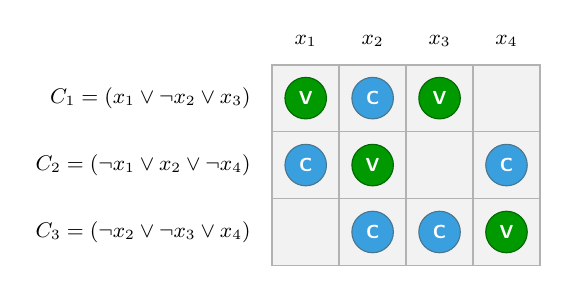
\begin{tikzpicture}[
    scale=0.85,
    transform shape,
    celda/.style={draw=gray!60, fill=gray!10, line width=0.6pt},
    verde/.style={circle, fill=green!60!black, draw=green!40!black, minimum size=0.62cm, inner sep=0pt, font=\footnotesize\sffamily\bfseries\color{white}},
    celeste/.style={circle, fill=cyan!75!blue!80, draw=cyan!50!black, minimum size=0.62cm, inner sep=0pt, font=\footnotesize\sffamily\bfseries\color{white}}
]
    \draw[celda] (0,0) rectangle (4,3);
    \draw[celda] (0,0) grid (4,3);

    % Encabezados de columnas (Variables)
    \node[font=\small\bfseries] at (0.5, 3.35) {$x_1$};
    \node[font=\small\bfseries] at (1.5, 3.35) {$x_2$};
    \node[font=\small\bfseries] at (2.5, 3.35) {$x_3$};
    \node[font=\small\bfseries] at (3.5, 3.35) {$x_4$};

    % Etiquetas de filas (Cláusulas)
    \node[anchor=east, font=\small] at (-0.2, 2.5) {$C_1 = (x_1 \lor \neg x_2 \lor x_3)$};
    \node[anchor=east, font=\small] at (-0.2, 1.5) {$C_2 = (\neg x_1 \lor x_2 \lor \neg x_4)$};
    \node[anchor=east, font=\small] at (-0.2, 0.5) {$C_3 = (\neg x_2 \lor \neg x_3 \lor x_4)$};

    % Piedras Fila 1
    \node[verde] at (0.5, 2.5) {V};
    \node[celeste] at (1.5, 2.5) {C};
    \node[verde] at (2.5, 2.5) {V};

    % Piedras Fila 2
    \node[celeste] at (0.5, 1.5) {C};
    \node[verde] at (1.5, 1.5) {V};
    \node[celeste] at (3.5, 1.5) {C};

    % Piedras Fila 3
    \node[celeste] at (1.5, 0.5) {C};
    \node[celeste] at (2.5, 0.5) {C};
    \node[verde] at (3.5, 0.5) {V};
\end{tikzpicture}


    \renewcommand{\thefigure}{3}
    \caption{Transformación polinomial de una instancia de 3-SAT a un tablero del Juego de las Piedras.}
    \label{fig:reduccion_3sat}
\end{figure}

Crear y llenar esta grilla de $n \times m$ leyendo las $n$ clausulas de $3$ literales cuesta $\mathcal{O}(n \cdot m)$ operaciones, por lo que \textbf{la reducción se ejecuta en tiempo polinomial}.

\noindent\textbf{Demostración de Equivalencia ($\iff$):} \\
Tenemos que probar que la formula 3-SAT $\mathcal{L}$ (la que tiene todo) es satisfacible \textbf{si y sólo si} el tablero $T$ construido tiene solución en el Juego de las Piedras.

\begin{itemize}
    \item \textbf{Ida ($\Rightarrow$): Si 3-SAT es satisfacible, entonces el tablero $T$ tiene solución.} \\
    Supongamos que existe una asignacion de verdad valida para $\mathcal{L}$. Para cada columna $j \in \{1, \dots, m\}$, hago en el tablero $T$:
    \begin{itemize}
        \item Si $x_j = \text{True}$, saco todas las piedras Celestes (\texttt{C}) de la columna $j$, quedandome solo con las Verdes (\texttt{V}).
        \item Si $x_j = \text{False}$, saco todas las piedras Verdes (\texttt{V}) de la columna $j$, quedandome solo con las Celestes (\texttt{C}).
    \end{itemize}
    Por la construccion, no va a haber columna que tenga piedras de los dos colores (se cumple la Regla 2 del problema). Además, como la asignación satisface $\mathcal{L}$, toda cláusula $C_i$ tiene al menos un literal verdadero. Si ese literal es positivo ($x_j = \text{True}$), en $T[i][j]$ había una piedra Verde que se quedó; si el literal es negado ($\neg x_j$ con $x_j = \text{False}$), en $T[i][j]$ había una piedra Celeste que también se quedó. Entonces, toda fila $i$ se queda con al menos una piedra (se cumple la Regla 1), obteniendo una solución válida para el Juego de las Piedras.

    \item \textbf{Vuelta ($\Leftarrow$): Si el tablero $T$ tiene solución, entonces 3-SAT es satisfacible.} \\
    Ahora suponemos que existe un conjunto de ``removidas'' valido en $T$ que cumple las dos reglas. Como ninguna columna $j$ tiene piedras de los dos colores en el tablero que queda, en cada columna $j$ quedan solo piedras Verdes, solo piedras celestes, o ninguna piedra. Definimos entonces la asignación booleana para cada variable $x_j$:
    \begin{itemize}
        \item Si en la columna $j$ quedaron piedras Verdes, ponemos $x_j = \text{True}$.
        \item Si en la columna $j$ quedaron piedras Celestes, ponemos $x_j = \text{False}$.
        \item Si la columna $j$ quedó completamente vacía, ponemos $x_j = \text{True}$.
    \end{itemize}
    Como la solución del tablero cumple la Regla 1, toda fila $i$ conserva al menos una piedra en alguna columna $j$. Si la piedra es Verde, por construcción el literal $x_j$ pertenecía a $C_i$ y nuestra asignación fijó $x_j = \text{True}$, haciendo verdadera a $C_i$. Si la piedra conservada es Celeste, el literal $\neg x_j$ pertenecía a $C_i$ y nuestra asignación fijó $x_j = \text{False}$, por lo que $\neg x_j = \text{True}$ y la cláusula $C_i$ también resulta verdadera. Así, las $n$ cláusulas se satisfacen simultáneamente.
\end{itemize}

Queda demostrado que $\text{3-SAT} \leq_P \text{Juego de las Piedras}$. Como el Juego de las Piedras $\in \mathcal{NP}$ y 3-SAT es NP-Completo, concluimos que \textbf{el Problema del Juego de las Piedras es NP-Completo}.







